\section{Why exact pair hulls do not compose}\label{sec:composition}

A solver that relaxes a quadratic expression term by term or pair by
pair works with the variables and products that occur in the model. Even
if every pair were relaxed exactly, the intersection of the pair hulls is
in general weaker than the hull of the joint graph. That gluing local
convex hulls along shared variables can fail is known, and the reason is
known as well: finitely many shared moments do not determine the shared
distribution \citep{Lasserre2006,NieDemmel2009,FantuzziFuentes2025}. This
section makes the phenomenon exact for the smallest quadratic case, a
path of three variables with exact pair hulls, and determines precisely
when gluing on a fixed number of shared moments fails. The results
explain why the merged blocks of Section~\ref{sec:quadratic} can be
stronger than their pairs, and they delimit that advantage.

\subsection{An example on a path}\label{sec:path-example}

Consider variables $x,y,z\in[0,1]$ that interact along the path
$x$--$y$--$z$. Write $m_u$ for the coordinate that represents $u$, $s_u$
for $u^2$ and $p_{uv}$ for $uv$. The exact pair hulls are
\[
H_{xy}=\conv\{(x,y,x^2,y^2,xy):x,y\in[0,1]\},\qquad
H_{yz}=\conv\{(y,z,y^2,z^2,yz):y,z\in[0,1]\},
\]
each of which is described by its semidefinite and RLT constraints
\citep{AnstreicherBurer2010}. Let $R$ be the set of points
$(m_x,m_y,m_z,s_x,s_y,s_z,p_{xy},p_{yz})$ whose $(x,y)$ and $(y,z)$ parts
lie in $H_{xy}$ and $H_{yz}$; the two parts share $m_y$ and $s_y$. The
joint hull $H=\conv\{(x,y,z,x^2,y^2,z^2,xy,yz):x,y,z\in[0,1]\}$ is
contained in $R$.

\begin{proposition}[A strict gap]\label{prop:path-gap}
The point
\begin{equation}\label{eq:witness}
\bar v=(m_x,m_y,m_z,s_x,s_y,s_z,p_{xy},p_{yz})
=\bigl(\tfrac12,\tfrac12,\tfrac45,\tfrac12,\tfrac5{16},\tfrac45,\tfrac38,\tfrac12\bigr)
\end{equation}
belongs to $R$ but not to $H$. The quadratic
\begin{equation}\label{eq:D-example}
D(x,y,z)=\bigl(y-\tfrac14-\tfrac x2\bigr)^2+\bigl(y-\tfrac{5z}8\bigr)^2+x(1-x)+z(1-z)
\end{equation}
has minimum $1/128$ on $[0,1]^3$, attained only at $(1,\tfrac{11}{16},1)$,
while its linearization vanishes at $\bar v$. The support inequality
\begin{equation}\label{eq:path-cut}
2s_y-\tfrac12m_y-p_{xy}-\tfrac54p_{yz}+\tfrac54m_x-\tfrac34s_x+m_z-\tfrac{39}{64}s_z\ \ge\ -\tfrac7{128}
\end{equation}
is valid for $H$ and violated by $1/128$ at $\bar v$.
\end{proposition}

\begin{proof}
The measure with mass $\tfrac12$ on each of $(x,y)=(0,\tfrac14)$ and
$(1,\tfrac34)$ has moments $(m_x,m_y,s_x,s_y,p_{xy})=(\tfrac12,\tfrac12,
\tfrac12,\tfrac5{16},\tfrac38)$. The measure with mass $\tfrac15$ on
$(y,z)=(0,0)$ and $\tfrac45$ on $(\tfrac58,1)$ has moments
$(m_y,m_z,s_y,s_z,p_{yz})=(\tfrac12,\tfrac45,\tfrac5{16},\tfrac45,\tfrac12)$.
They agree on $(m_y,s_y)$, so $\bar v\in R$. The two pair parts of $D$,
$(y-\tfrac14-\tfrac x2)^2+x(1-x)$ and $(y-\tfrac{5z}8)^2+z(1-z)$, vanish on
the supports of the respective measures, so the linearization of $D$
vanishes at $\bar v$. The minimum is the case $A=\{\tfrac14,\tfrac34\}$,
$C=\{0,\tfrac58\}$ of Theorem~\ref{thm:interleave}, with
$\delta=\tfrac34-\tfrac58=\tfrac18$. Expanding $D\ge\tfrac1{128}$ gives
\eqref{eq:path-cut}, since the constant term of $D$ is $\tfrac1{16}$.
\end{proof}

The inequality~\eqref{eq:path-cut} uses only coordinates that occur in the
model; it needs no product $xz$. It is the support inequality of the
three-variable block in the direction of $D$, so both oracles of
Section~\ref{sec:quadratic} compute it exactly.

\subsection{An exact description for the path family}\label{sec:interleave}

The example belongs to a family whose behavior can be described
completely. Fix an interval $[\ell,u]$ for $y$ and two-point sets
$A=\{a_1,a_2\}$ and $C=\{c_1,c_2\}$ in $[\ell,u]$ with $a_1\ne a_2$ and
$c_1\ne c_2$. For weights $\omega_A\ge(a_2-a_1)^2$ and
$\omega_C\ge(c_2-c_1)^2$ let
\begin{equation}\label{eq:family}
D_A(x,y)=\bigl(y-a_1-(a_2-a_1)x\bigr)^2+\omega_Ax(1-x),\qquad
D_C(y,z)=\bigl(y-c_1-(c_2-c_1)z\bigr)^2+\omega_Cz(1-z),
\end{equation}
with $x,z\in[0,1]$, and $D=D_A+D_C$. Let $R$ be defined as above, on the
box $[0,1]\times[\ell,u]\times[0,1]$, and let
$\delta=\min\{\abs{s-t}:s\in A,\ t\in C\}$. The sets $A$ and $C$
\emph{interleave} if they are disjoint and their elements alternate in
sorted order.

\begin{theorem}[Interleaving]\label{thm:interleave}
\begin{enumerate}[label=(\roman*)]
\item The minimum of $D$ over the box is $\delta^2/2$.
\item The minimum of the linearization of $D$ over $R$ is $0$ if
$A\cap C\ne\emptyset$ or $A$ and $C$ interleave, and $\delta^2/2$ otherwise.
\end{enumerate}
The gap between $H$ and $R$ in the direction of $D$ is therefore either
$0$ or $\delta^2/2$; it is $\delta^2/2$ exactly when $A$ and $C$
interleave.
\end{theorem}

\begin{proof}
Since $\omega_A\ge(a_2-a_1)^2$, the function $D_A(\cdot,y)$ is concave or
affine, so its minimum over $[0,1]$ is attained at $x\in\{0,1\}$, where it
equals $(y-a_1)^2$ or $(y-a_2)^2$. Hence
$\min_{x\in[0,1]}D_A(x,y)=\dist(y,A)^2$, and similarly for $D_C$.

(i) For fixed $y$ the minimum over $x$ and $z$ is
$\min_{s\in A,t\in C}\{(y-s)^2+(y-t)^2\}$, and
$(y-s)^2+(y-t)^2=2(y-\tfrac{s+t}2)^2+\tfrac12(s-t)^2$ with
$\tfrac{s+t}2\in[\ell,u]$.

(ii) A point of $H_{xy}$ is the moment vector of a finitely supported
probability measure $\pi$ on $[0,1]\times[\ell,u]$, and the linearization
of $D_A$ at that point is $\int D_A\,d\pi\ge\int\dist(y,A)^2\,d\nu$, where
$\nu$ is the $y$-marginal of $\pi$; equality holds when $\pi$ puts its mass
at a minimizing $x\in\{0,1\}$ for each $y$. Hence the minimum over $R$ is
the minimum of $\int\dist(y,A)^2\,d\nu_A+\int\dist(y,C)^2\,d\nu_C$ over
probability measures $\nu_A,\nu_C$ on $[\ell,u]$ with equal first and
second moments. It is zero if and only if some measure on $A$ and some
measure on $C$ have equal first two moments, that is, if the chords of the
parabola $\{(t,t^2)\}$ spanned by $A$ and by $C$ meet. Two such chords meet
if they share an endpoint; otherwise, since no three points of a parabola
are collinear and $(t,t^2)$ lies below the chord spanned by $A$ exactly
when $t$ lies between $a_1$ and $a_2$, they meet if and only if $A$ and $C$
interleave. When the chords do not meet, $A$ and $C$ are either separated
(one lies below the other) or nested (one lies between the two points of
the other). In both cases Appendix~\ref{app:interleave} gives a polynomial
$p$ of degree at most two such that $\dist(y,A)^2-p(y)\ge\kappa_A$ and
$\dist(y,C)^2+p(y)\ge\kappa_C$ for all $y$, with $\kappa_A+\kappa_C=\delta^2/2$.
Integrating against $\nu_A$ and $\nu_C$, whose moments of order at most
two agree, shows that the minimum over $R$ is at least $\delta^2/2$, and
graph points show that it is at most $\delta^2/2$.
\end{proof}

\begin{figure}[t]
\centering
\begin{tikzpicture}[scale=4.2]
\begin{scope}
\draw[->] (-0.05,0) -- (0.9,0) node[right] {$t$};
\draw[->] (0,-0.03) -- (0,0.78) node[above] {$t^2$};
\draw[thick,gray,domain=-0.02:0.86,smooth,variable=\t] plot ({\t},{\t*\t});
\coordinate (a1) at (0.25,0.0625); \coordinate (a2) at (0.75,0.5625);
\coordinate (c1) at (0,0); \coordinate (c2) at (0.625,0.390625);
\draw[very thick,blue] (a1) -- (a2);
\draw[very thick,red,dashed] (c1) -- (c2);
\fill[blue] (a1) circle (0.012) node[below right] {$\tfrac14$};
\fill[blue] (a2) circle (0.012) node[right] {$\tfrac34$};
\fill[red] (c1) circle (0.012) node[below left] {$0$};
\fill[red] (c2) circle (0.012) node[above left] {$\tfrac58$};
\fill (0.5,0.3125) circle (0.014);
\node[anchor=north west] at (0.52,0.30) {\small $(\tfrac12,\tfrac5{16})$};
\node at (0.42,0.72) {\small (a) interleaving};
\end{scope}
\begin{scope}[xshift=1.15cm]
\draw[->] (-0.05,0) -- (0.9,0) node[right] {$t$};
\draw[->] (0,-0.03) -- (0,0.78) node[above] {$t^2$};
\draw[thick,gray,domain=-0.02:0.86,smooth,variable=\t] plot ({\t},{\t*\t});
\coordinate (a1) at (0,0); \coordinate (a2) at (0.75,0.5625);
\coordinate (c1) at (0.25,0.0625); \coordinate (c2) at (0.5,0.25);
\draw[very thick,blue] (a1) -- (a2);
\draw[very thick,red,dashed] (c1) -- (c2);
\fill[blue] (a1) circle (0.012) node[below left] {$0$};
\fill[blue] (a2) circle (0.012) node[right] {$\tfrac34$};
\fill[red] (c1) circle (0.012) node[below right] {$\tfrac14$};
\fill[red] (c2) circle (0.012) node[below right] {$\tfrac12$};
\node at (0.42,0.72) {\small (b) nested};
\end{scope}
\end{tikzpicture}
\caption{Moment pairs $(\E y,\E y^2)$ of distributions on a two-point set
form the chord of the parabola between the two points. Solid: $A$;
dashed: $C$. (a) The sets $A=\{\tfrac14,\tfrac34\}$ and $C=\{0,\tfrac58\}$ of
Proposition~\ref{prop:path-gap} interleave,
the chords cross at $(\tfrac12,\tfrac5{16})$, and the glued pair relaxation
has value $0$. (b) Nested sets $A=\{0,\tfrac34\}$ and $C=\{\tfrac14,\tfrac12\}$:
the chords do not meet, and by
Theorem~\ref{thm:interleave} the glued relaxation attains the true minimum
$\delta^2/2$ in the direction of $\Phi$.}
\label{fig:chords}
\end{figure}


Proposition~\ref{prop:path-gap} is the case $[\ell,u]=[0,1]$,
$A=\{\tfrac14,\tfrac34\}$, $C=\{0,\tfrac58\}$ and $\omega_A=\omega_C=1$,
with sorted order $0,\tfrac14,\tfrac58,\tfrac34$. The theorem also shows
what goes wrong. In $R$ the two pairs may represent $y$ by different
distributions that agree only in their first two moments. Each pair
places $y$ on its own preferred two-point set, and whenever the chords
cross, the two distributions have the same mean and second moment.

\subsection{Matching more moments}\label{sec:k-moments}

The same mechanism defeats any interface that identifies a fixed finite
number of moments of the shared variable. Let $K_L$ and $K_R$ be compact
sets of points $(x,y)$ and $(y,z)$, with $y$ scalar, and let $H_L$ and
$H_R$ be the convex hulls of continuous feature maps on them whose first
$k$ coordinates are $y,y^2,\dots,y^k$; the other local features are
arbitrary. Let $R_k$ be the set of pairs of points of $H_L$ and $H_R$ that
agree in these $k$ coordinates. Let $D_L\ge0$ and $D_R\ge0$ be affine
in the local features, with zero sets $Z_L$ and $Z_R$, and let $A$ and
$C$ be the projections of $Z_L$ and $Z_R$ onto $y$. For disjoint compact
$A,C\subset\R$, the \emph{alternation number} $\mathrm{alt}(A,C)$ is the
largest $r$ for which there are points $t_0<\dots<t_r$ of $A\cup C$ with
consecutive points in different sets.

\begin{theorem}[Alternation]\label{thm:alternation}
Suppose $A$ and $C$ are disjoint, so that $D_L+D_R>0$ on the joint
domain. The linearization of $D_L+D_R$ vanishes at some point of $R_k$ if
and only if $\mathrm{alt}(A,C)\ge k+1$. In particular, gluing on $k$
moments always detects the gap when $\abs A+\abs C\le k+1$, and, for
finite sets with $\abs A+\abs C=k+2$, fails to detect it exactly when $A$
and $C$ alternate.
\end{theorem}

\begin{proof}
As in the proof of Theorem~\ref{thm:interleave}, the linearization
vanishes at a point of $R_k$ if and only if there are probability measures
on $A$ and on $C$ with equal moments of orders $1,\dots,k$; these measures
lift to $Z_L$ and $Z_R$ atom by atom. If $\mathrm{alt}(A,C)=r\le k$, there is
a polynomial of degree $r$ that is positive on $A$ and negative on $C$
(it changes sign once in each gap between consecutive runs of $A\cup C$;
Appendix~\ref{app:alternation}), and its integrals against two such
measures would have to be equal, a contradiction. If
$\mathrm{alt}(A,C)\ge k+1$, take an alternating chain $t_0<\dots<t_{k+1}$
and the weights $\sigma_i=\prod_{j\ne i}(t_i-t_j)^{-1}$ of the divided
difference of order $k+1$. They annihilate all polynomials of degree at
most $k$, and their signs alternate, so their positive and negative parts,
normalized, are probability measures on the $A$-points and on the
$C$-points with equal moments of orders $0,\dots,k$.
\end{proof}

The criterion is a consequence of the classical fact that a signed
measure annihilating the polynomials of degree at most $k$ changes sign at
least $k+1$ times \citep{KarlinStudden1966}. Its use here is to identify
exactly which configurations escape a $k$-moment interface. Every $k$ is
defeated by some quadratic configuration.

\begin{proposition}[A full gap for every $k$]\label{prop:full-gap}
Let $r\ge1$ and $k\le2^{r+1}-2$. On $x,z\in[0,1]^r$ and
$y\in[0,2^{r+1}-1]$ let
\[
D_L=\Bigl(y-\sum_{j=1}^r2^jx_j\Bigr)^2+\sum_{j=1}^r4^jx_j(1-x_j),\qquad
D_R=\Bigl(y-1-\sum_{j=1}^r2^jz_j\Bigr)^2+\sum_{j=1}^r4^jz_j(1-z_j).
\]
Then $\min(D_L+D_R)=1/2$, while the linearization of $D_L+D_R$ vanishes at
a point of $R_k$, for local hulls of the features $y,\dots,y^{\max\{k,2\}}$,
$x_j$, $yx_j$, $x_ix_j$ and their analogues for $z$.
\end{proposition}

\begin{proof}
$D_L$ is multilinear in $x$, so its minimum over $x$ is attained at a
vertex, where it equals $(y-2\sum_{j\in J}2^{j-1})^2$ for a subset $J$; hence
$\min_xD_L=\dist(y,A)^2$ with $A=\{0,2,\dots,2^{r+1}-2\}$, and similarly
$\min_zD_R=\dist(y,C)^2$ with $C=\{1,3,\dots,2^{r+1}-1\}$. Thus $\delta=1$ and
the minimum is $1/2$ as in Theorem~\ref{thm:interleave}(i). The points
$0,1,\dots,k+1$ alternate between $A$ and $C$, so Theorem~\ref{thm:alternation}
applies; explicitly, the binomial weights $\binom{k+1}i2^{-k}$ on the even
and on the odd integers $i\le k+1$ have equal moments of orders up to $k$.
\end{proof}

Thus no fixed number of shared moments makes the gluing exact, even for
quadratic blocks, and the relative gap can be $100\%$. As $k\to\infty$ the
glued bounds do converge to the true minimum, because measures on a
compact interval are determined by their moments and measures with equal
marginals glue \citep[Lemma~6.3]{Lasserre2006}; the convergence is not
uniform over instances.

\subsection{Relation to known results}\label{sec:composition-literature}

Several earlier examples show that sparse relaxations on a path can be
strictly weaker than dense ones. \citet[Example~3.5]{NieDemmel2009} give a
numerical quartic example, and \citet[Example~6.7]{NieQuTangZhang2026} a
box-constrained quartic for which the sparse moment hierarchy is never
tight. Finite gluing results require additional rank or flatness
conditions on the overlaps \citep[Theorem~3.7]{Lasserre2006},
\citep{FantuzziFuentes2025}. For quadratic problems with sign-oriented
squares, \citet[Corollary~1]{DeyKhajavirad2025} decompose the convex hull
across a complete separator that carries no positive square term (no
``plus loop''), and \citet{Khajavirad2026} builds on this decomposition.
Proposition~\ref{prop:path-gap} shows that this hypothesis cannot be
dropped even for a path of three variables with a single plus loop at the
center: the reduced objective
$2y^2-\tfrac12y-xy-\tfrac54yz+\tfrac1{16}+\tfrac12x+\tfrac{25}{64}z$, which
equals $D$ at binary leaves, has the same witness and the same gap
$1/128$. To our knowledge, a degree-two example with exact pair hulls, an
exact rational gap, a separating cut in the existing coordinates, and the
exact characterizations of Theorems~\ref{thm:interleave}
and~\ref{thm:alternation} have not been given before.

The advantage of the joint block over its pairs does not extend to dense
relaxations. On the whole family~\eqref{eq:family}, with $u=y-a_1-(a_2-a_1)x$
and $v=y-c_1-(c_2-c_1)z$,
\begin{equation}\label{eq:sdp-identity}
D-\frac{\delta^2}2=\frac{(u+v)^2}2+\sum_{i,j\in\{0,1\}}F_{ij}\,\ell_{ij}(x,z)
+\Bigl(\omega_A-\frac{(a_2-a_1)^2}2\Bigr)x(1-x)+\Bigl(\omega_C-\frac{(c_2-c_1)^2}2\Bigr)z(1-z),
\end{equation}
where $\ell_{00}=(1-x)(1-z)$, $\ell_{10}=x(1-z)$, $\ell_{01}=(1-x)z$,
$\ell_{11}=xz$, and $F_{ij}=\tfrac12\bigl((c_{j+1}-a_{i+1})^2-\delta^2\bigr)\ge0$.
The linearized $\ell_{ij}$ are the McCormick expressions of the product
$xz$, the linearized $(u+v)^2$ is a quadratic form in the dense moment
matrix of $(1,x,y,z)$, and the last two terms are nonnegative on the pair
hulls. Hence the dense moment matrix together with the McCormick
inequalities of the \emph{nonedge} product $xz$ proves $D\ge\delta^2/2$ for
every member of the family; neither ingredient alone suffices
(Appendix~\ref{app:sdp}). This is consistent with a theorem of
\citet[Theorem~1]{BurerNatarajanWillemsen2025}: for box-constrained
quadratic programs in at most three variables whose off-diagonal
coefficients are nonpositive, a semidefinite relaxation with part of the
RLT inequalities is exact. After an affine change of $y$ to $[0,1]$ and,
if necessary, the complements $1-x$ and $1-z$, every member of the family
has this sign pattern. The support
inequality~\eqref{eq:path-cut} attains the same bound without the
coordinate $p_{xz}$ and without a semidefinite constraint. That matters in
practice, because solvers relax the products present in the model and
rarely add new ones, but it is an advantage of representation, not of
strength.

\subsection{When composition is exact, and the gain from merging}\label{sec:gluing}

Gluing is exact when the shared coordinates determine the shared
distribution. Under a running-intersection decomposition, local measures
with equal full marginals on the separators glue to a global measure
\citep{Vorobev1962,Lasserre2006}. If the separator takes at most $r$
known values, its moments of orders $0,\dots,r-1$ determine its
distribution through a Vandermonde system; for a binary separator the mean
suffices. This is why the McCormick inequalities describe the convex hull
of a pure bilinear function on a forest over the unit box
\citep[Proposition~8]{Padberg1989}: the extreme points are binary, the
McCormick inequalities of an edge are the nonnegativity of the four joint
probabilities of its endpoints, and adjacent edges share a binary variable
whose distribution is fixed by its mean. Square terms break this argument,
because they let a fractional mean be realized by continuous
distributions, as in~\eqref{eq:witness}.

Finally, the gain from merging pair directions into one star direction
can be computed exactly.

\begin{corollary}[Gain from merging]\label{cor:gain}
Let $P_i\subset\R^2$ be compact polytopes in the variables $(y,x_i)$,
$i=1,\dots,k$, whose star domain $S=\{(y,x):(y,x_i)\in P_i\ \forall i\}$ is
nonempty, and let $q_i(y,x_i)$ be quadratics. Put $\beta_i=\min_{P_i}q_i$,
$\beta^\ast=\min_S\sum_iq_i$ and $\Delta=\beta^\ast-\sum_i\beta_i$. Then
$\Delta\ge0$ is the largest constant by which the sum of the $k$ pair
inequalities $q_i\ge\beta_i$ can be improved in the direction $\sum_iq_i$,
and $\Delta>0$ if and only if the projections onto $y$ of the sets
$\argmin_{P_i}q_i$ have empty common intersection.
\end{corollary}

\begin{proof}
Clearly $\sum_iq_i\ge\sum_i\beta_i$ on $S$, and $\beta^\ast$ is the best
constant in that direction. If some $\bar y$ lies in every projection,
choose $x_i$ with $(\bar y,x_i)\in\argmin_{P_i}q_i$; the assembled point
lies in $S$ and attains $\sum_i\beta_i$. Conversely, if $\Delta=0$, a
minimizer over $S$, which exists by compactness, minimizes every $q_i$,
so its $y$-coordinate lies in every projection.
\end{proof}

Both $\beta_i$ and $\beta^\ast$ are computed exactly by the algorithms of
Section~\ref{sec:quadratic}; in Proposition~\ref{prop:path-gap} both pair
minima are zero and $\Delta=1/128$. Pairwise intersections of the
projections are not enough: they can all be nonempty while $\Delta>0$.
The quantity $\Delta$ compares the merged cut with separately added pair
cuts. The gap to the glued relaxation $R$ lies in $[0,\Delta]$ and can be
smaller: for $A=\{0,3\}$ and $C=\{1,2\}$ on $y\in[0,3]$, a nested
configuration, $\Delta=1/2$ but the gap to $R$ is zero by
Theorem~\ref{thm:interleave}. The corollary is a diagnostic for a proposed
merge; it does not say which directions to merge or whether merging pays
off in a solver.
